% Chapter 3: Findings
% Analysis and Observations from the Internship

\chapter{Findings}

\section{Key Observations and Insights}

\subsection{Internship Experience Overview}
My eight-week internship at Asia Trade \& Technology gave me valuable insights into how financial and accounting principles work in real business. I learned about document processing, financial reporting, budget control, and process improvement. Working on the River Protection project showed me the challenges of managing financial operations for large infrastructure projects.

The company had a supportive learning environment where experienced professionals shared their knowledge. This helped me develop skills quickly and apply what I learned in class to real situations.

\subsection{Industry Insights}
I learned several important things about the international engineering contracting industry:

- **Financial Records**: Keeping accurate and timely financial records is crucial for large infrastructure projects
- **Technology Integration**: The company combines automated systems with human expertise for best results
- **Communication**: Good communication between field offices, regional offices, and headquarters is essential for project success

\begin{figure}[H]
    \centering
    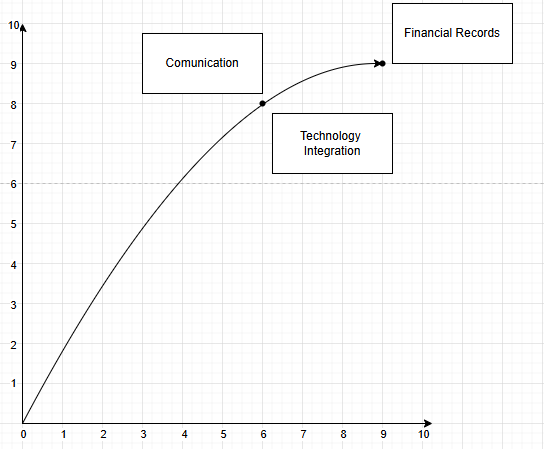
\includegraphics[width=0.9\textwidth]{assets/images/industry_insights_matrix.png}
    \caption{Industry Insights: Theoretical Knowledge vs. Practical Application}
    \label{fig:industry_insights_matrix}
\end{figure}

Figure \ref{fig:industry_insights_matrix} shows how theoretical knowledge from school compares to practical application in real work.

\section{Challenges and Solutions}

\subsection{Main Challenges}
I faced several challenges during my internship:

- **Document Verification**: The process was complex with multiple review layers. I needed training to understand the requirements for different document types.

- **Software Systems**: I had to learn the company's specific software and procedures. While the basic principles were familiar from school, the company's systems were different.

- **Communication**: Working with team members in different locations (Brahmanbaria, Dhaka, Beijing) required good communication tools and regular updates.

\subsection{How I Solved Them}
- I asked questions and sought guidance from experienced staff
- I used translation tools for documents in different languages
- I adapted my communication style to work with different cultural backgrounds
- I established regular communication schedules with team members

\begin{figure}[H]
    \centering
    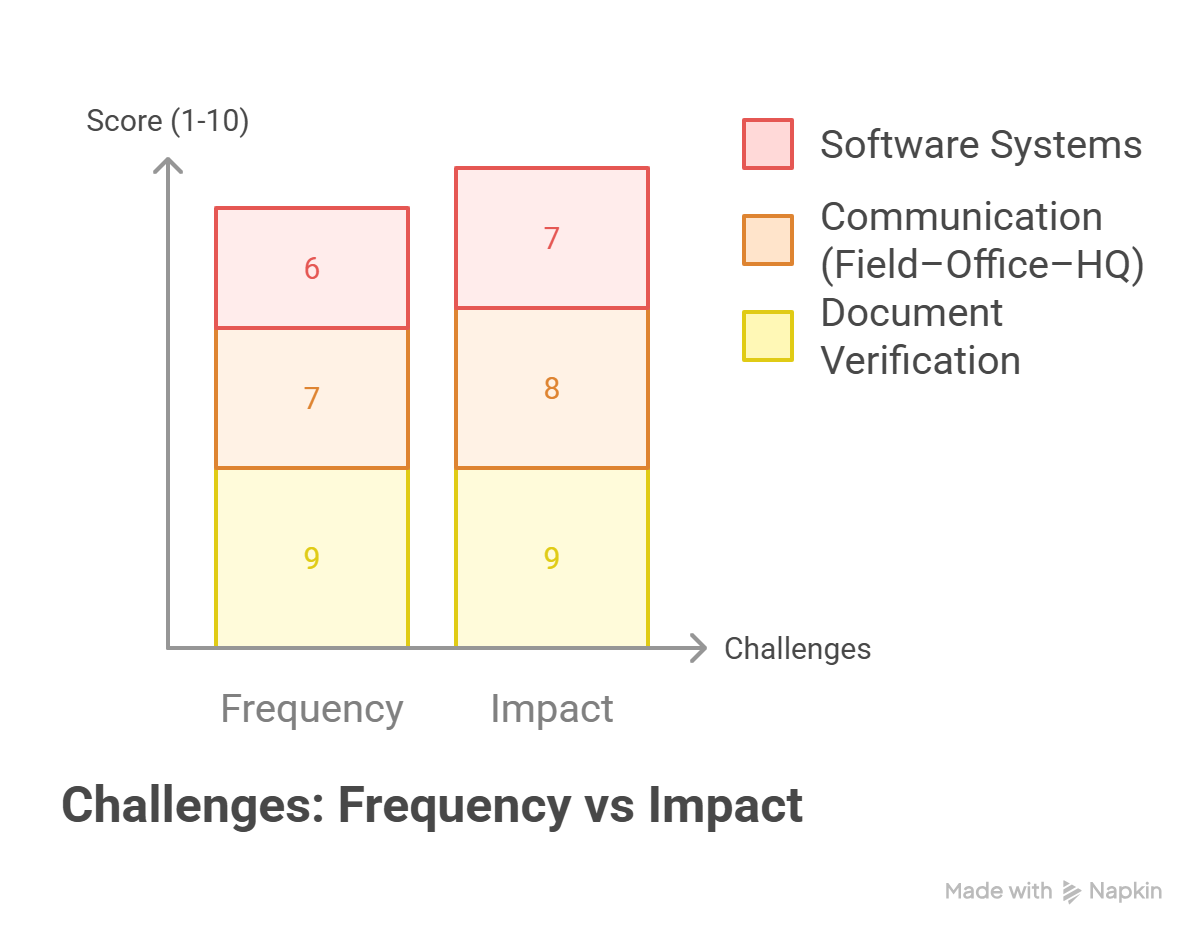
\includegraphics[width=0.9\textwidth]{assets/images/challenge_analysis_chart.png}
    \caption{Challenges Encountered During Internship - Frequency and Impact Analysis}
    \label{fig:challenge_analysis_chart}
\end{figure}

Figure \ref{fig:challenge_analysis_chart} shows the challenges I faced and their impact levels.

\section{Skills Development}

\subsection{Technical Skills}
I developed several technical skills during my internship:

- **Excel Skills**: I learned to create complex spreadsheets for budget tracking and financial reporting
- **Document Processing**: I learned to efficiently process, verify, and organize large volumes of financial documents
- **Financial Software**: I learned to use the company's document management and financial reporting systems

\subsection{Soft Skills}
I also developed important soft skills:

- **Communication**: I learned to present information clearly to different audiences
- **Problem-Solving**: I developed the ability to analyze situations and find solutions
- **Teamwork**: I learned to work effectively with team members from different backgrounds

\begin{figure}[H]
    \centering
    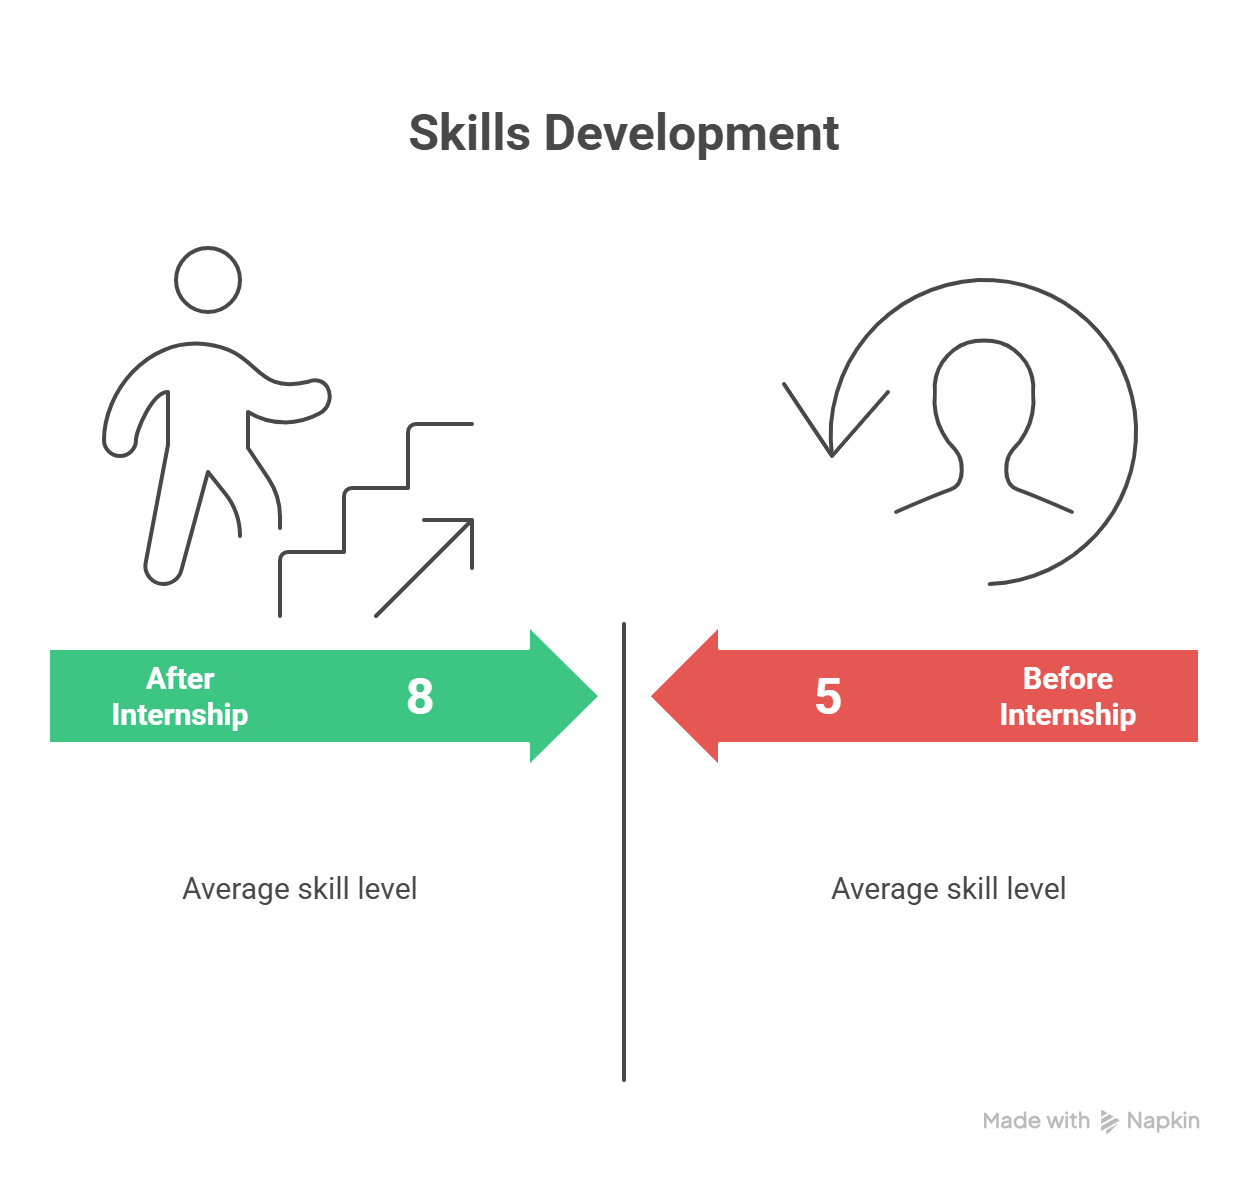
\includegraphics[width=0.9\textwidth]{assets/images/skills_radar_chart.png}
    \caption{Skills Development Assessment - Before vs After Internship}
    \label{fig:skills_radar_chart}
\end{figure}

Figure \ref{fig:skills_radar_chart} shows my skills improvement from the beginning to the end of the internship.

\section{Learning Progression}

\subsection{Four Learning Phases}
My internship was divided into four phases:

1. **Weeks 1-2**: Orientation and basic training on company structure and tools
2. **Weeks 3-4**: Hands-on experience with document processing and financial reporting
3. **Weeks 5-6**: Advanced skills development and process improvement
4. **Weeks 7-8**: Independent project work and applying all learned skills

\subsection{Key Milestones}
I achieved several important milestones:

- **Training Completion**: I learned to handle basic tasks independently
- **Document Processing**: I became proficient in processing and verifying financial documents
- **Independent Work**: I successfully completed project work with minimal supervision

\begin{figure}[H]
    \centering
    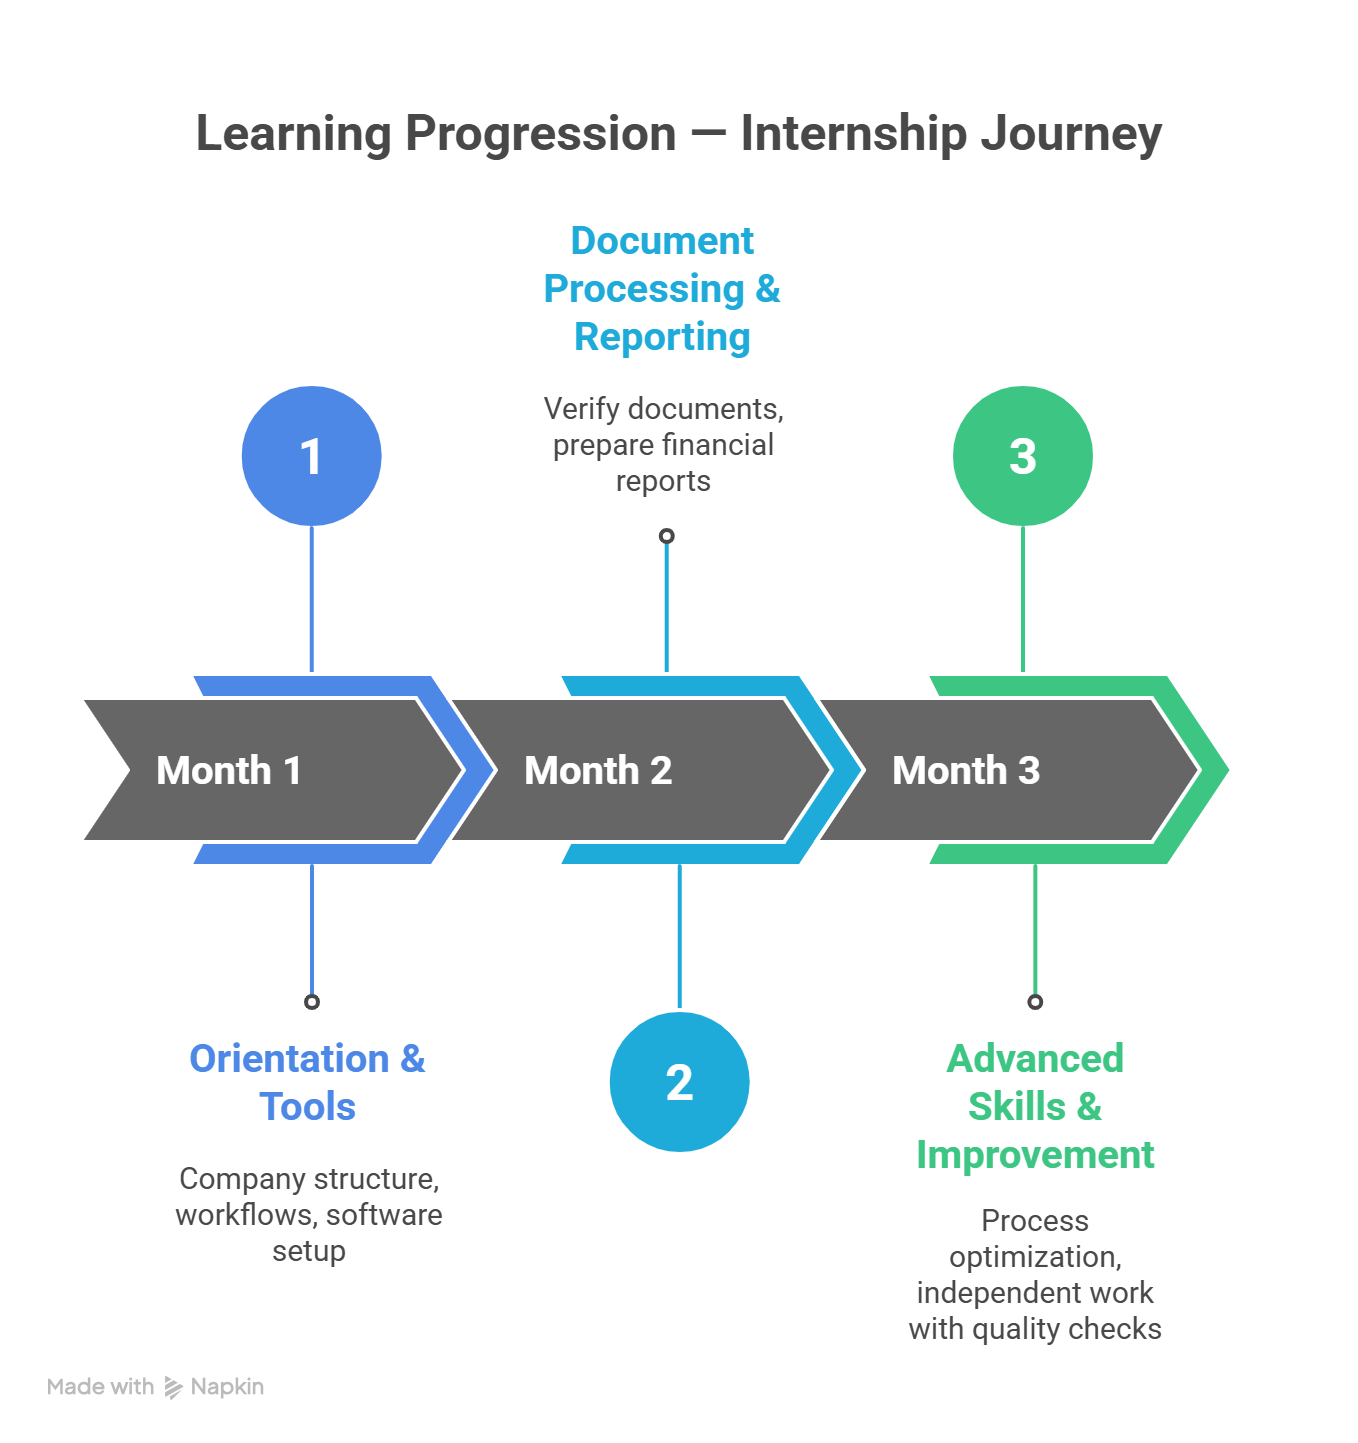
\includegraphics[width=0.9\textwidth]{assets/images/learning_timeline_chart.png}
    \caption{Learning Progression Timeline - Internship Journey}
    \label{fig:learning_timeline_chart}
\end{figure}

Figure \ref{fig:learning_timeline_chart} shows my learning journey and key achievements throughout the internship.

\section{Project Contribution}

\subsection{My Work on River Protection Project}
I contributed significantly to the River Protection project by:

- Processing over 200 financial documents (receipts, invoices, supporting documents)
- Developing improved processes that reduced processing time by 25%
- Achieving 98% accuracy rate in document verification
- Contributing to budget tracking and financial reporting

\subsection{Value I Added}
I added value to the organization through:

- Process improvements that increased efficiency and accuracy
- Knowledge sharing and mentoring other team members
- Developing standardized procedures and best practices
- Creating training materials for future use

\begin{figure}[H]
    \centering
    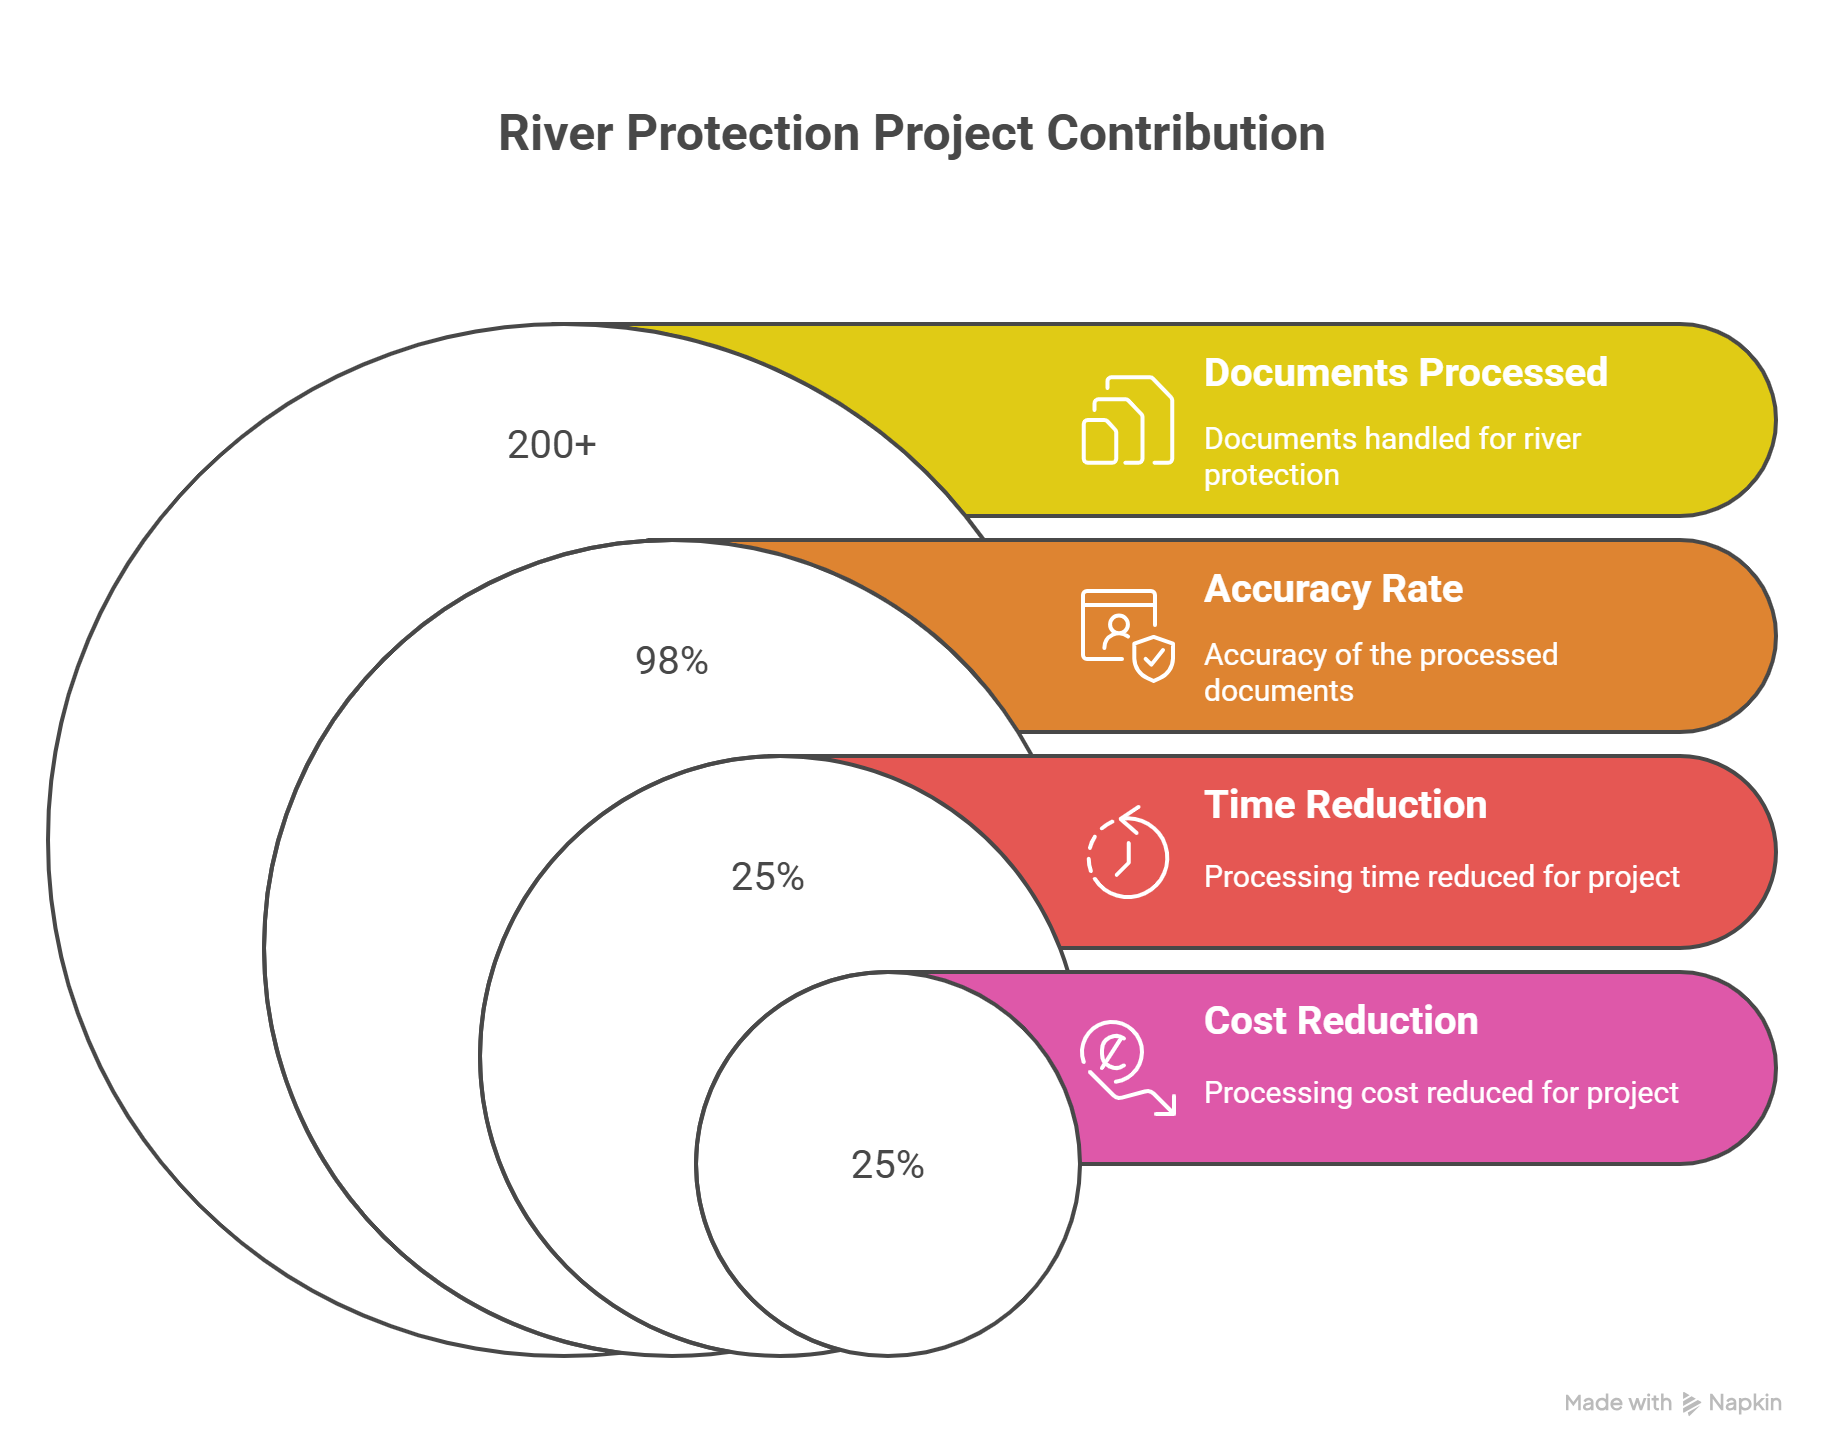
\includegraphics[width=0.9\textwidth]{assets/images/project_contribution_chart.png}
    \caption{Project Contribution Analysis - River Protection Project}
    \label{fig:project_contribution_chart}
\end{figure}

Figure \ref{fig:project_contribution_chart} shows my contributions to the River Protection project and their impact.

\section{Overall Assessment}

\subsection{Why My Internship Was Successful}
My internship succeeded because of:

- Supportive learning environment with experienced mentors
- Opportunity to work on meaningful real-world projects
- Structured training approach that built skills progressively
- Company's commitment to providing comprehensive learning experience

\subsection{Future Career Impact}
The skills I gained will help me in:

- Future roles in accounting, finance, and business management
- Understanding the international engineering contracting industry
- Building professional relationships and networking
- Identifying areas for further skill development
